\documentclass[a4paper,oneside,12pt]{article}

\usepackage[slovene]{babel}    % slovenian language and hyphenation
\usepackage[utf8]{inputenc}    % make čšž work on input
\usepackage[T1]{fontenc}       % make čšž work on output
\usepackage[reqno]{amsmath}    % basic ams math environments and symbols
\usepackage{amssymb,amsthm}    % ams symbols and theorems
\usepackage{mathtools}         % extends ams with arrows and stuff
\usepackage{url}               % \url and \href for links
\usepackage{icomma}            % make comma a thousands separator with correct spacing
\usepackage{units}             % \unit[1]{m} and unitfrac
\usepackage{enumerate}         % enumerate style
\usepackage{array}             % mutirow
\usepackage[usenames]{color}   % colors with names
\usepackage{graphicx}          % images

\usepackage[bookmarks, colorlinks=true, linkcolor=black, anchorcolor=black,
  citecolor=black, filecolor=black, menucolor=black, runcolor=black,
  urlcolor=black, pdfencoding=unicode]{hyperref}  % clickable references, pdf toc
\usepackage[
  paper=a4paper,
  top=1cm,
  bottom=1cm,
  left=1cm,
  right=1cm
% textheight=24cm,
]{geometry}  % page geomerty

\newtheorem{izrek}{Izrek}
\newtheorem{posledica}{Posledica}

\theoremstyle{definition}
\newtheorem{definicija}{Definicija}
\newtheorem{opomba}{Opomba}
\newtheorem{zgled}{Zgled}

% basic sets
\newcommand{\R}{\ensuremath{\mathbb{R}}}
\newcommand{\N}{\ensuremath{\mathbb{N}}}
\newcommand{\Z}{\ensuremath{\mathbb{Z}}}
\renewcommand{\C}{\ensuremath{\mathbb{C}}}
\newcommand{\Q}{\ensuremath{\mathbb{Q}}}
\newcommand{\M}{\ensuremath{\mathcal{M}}}

% greek letters
\let\oldphi\phi
\let\oldtheta\theta
\newcommand{\eps}{\varepsilon}
\renewcommand{\phi}{\varphi}
\renewcommand{\theta}{\vartheta}

% vektorska analiza
\newcommand{\grad}{\operatorname{grad}}
\newcommand{\rot}{\operatorname{rot}}
\renewcommand{\div}{\operatorname{div}}

% lists with less vertical space
\newenvironment{itemize*}{\vspace{-1.8\parskip}\begin{itemize}\setlength{\itemsep}{0pt}\setlength{\parskip}{2pt}}{\end{itemize}\vspace{-1\parskip}}
\newenvironment{enumerate*}{\vspace{-1.8\parskip}\begin{enumerate}\setlength{\itemsep}{0pt}\setlength{\parskip}{2pt}}{\end{enumerate}\vspace{-1\parskip}}
\newenvironment{description*}{\vspace{-6pt}\begin{description}\setlength{\itemsep}{0pt}\setlength{\parskip}{2pt}}{\end{description}\vspace{-1\parskip}}

\newcommand{\Title}{}
\newcommand{\Author}{Jure Slak}
\title{\Title}
\author{\Author}
\date{\today}
\hypersetup{pdftitle={\Title}, pdfauthor={\Author}, pdfcreator={\Author},
            pdfproducer={\Author}, pdfsubject={}, pdfkeywords={}}  % setup pdf metadata

% \pagestyle{empty}              % vse strani prazne
\setlength{\parindent}{0pt}    % zamik vsakega odstavka
\setlength{\parskip}{4pt}     % prazen prostor po odstavku
% \setlength{\overfullrule}{30pt}  % oznaci predlogo vrstico z veliko črnine

\usepackage{titlesec}
\titleformat*{\section}{\large\bfseries}
\titleformat*{\subsection}{\large\bfseries}
\titleformat*{\subsubsection}{\bfseries}
\titlespacing*{\section}{0pt}{0pt}{-4pt}   % left, before, after
\titlespacing*{\subsection}{0pt}{1pt}{-1pt}

\pagestyle{empty}

\newbox\gnBoxA
\newdimen\gnCornerHgt
\setbox\gnBoxA=\hbox{$\ulcorner$}
\global\gnCornerHgt=\ht\gnBoxA
\newdimen\gnArgHgt
\def\Godelnum #1{%
\setbox\gnBoxA=\hbox{$#1$}%
\gnArgHgt=\ht\gnBoxA%
\ifnum     \gnArgHgt<\gnCornerHgt \gnArgHgt=0pt%
\else \advance \gnArgHgt by -\gnCornerHgt%
\fi \raise\gnArgHgt\hbox{$\ulcorner$} \box\gnBoxA %
\raise\gnArgHgt\hbox{$\urcorner$}}

\DeclareMathOperator{\Th}{Th}
\DeclareMathOperator{\Ar}{Ar}
\DeclareMathOperator{\FV}{FV}
\newcommand{\Prf}{\mathsf{Prf}}
\newcommand{\Prov}{\mathsf{Prov}}
\newcommand{\Con}{\mathsf{Con}}

\begin{document}

% \thispagestyle{empty}  % ta stran prazna

% za na list (iz online skripte logic.pdf):
% stran 19 v celoti
% stran 4 zgornji del NEEEEEEEEEE
% stran 6, lema 2.1 --> Tega pa ne bomo kot sliko dali noter...
% pravila za Hilbertov sistem (uno z vaj)
% Jure, sej to lahko vstavimo kot slike ane?
% ## Ja, bom jaz.
% Trenutno mi ne uspe uploadat fileov...

% Lema 2.1 (daj jo kamor želiš - bomo na koncu nekam vrgl, to je uporabno pri dokazvanju soundnessa):
% $u[t/x]_{\M}^\rho = u^{\rho[t^\rho_\M/x]}_{\M}$, and $M \models (A[t/x])^\rho$ iff $M \models A^{\rho[x\mapsto t^\rho_\M]}$.

% like :D :D
% Za G\"odla: $\Godelnum{A}$ $\Godelnum{ \phi \Godelnum{\Godelnum{3}^5}}$.

% \section*{Some general stuff}

\textbf{Def: }
$(\mathcal{F}, \mathcal{P})$ is a \emph{signature}, where
$\mathcal{F}$ -- set of \emph{function symbols},
$\mathcal{P}$ -- set of \emph{predicate symbols}.
Each $f \in \mathcal{F}$ and $P \in \mathcal{P}$ has an associated \emph{arity} $\Ar(f)$ or $\Ar(P)$.\\
\textbf{Syntax:}
A \textbf{term} $t$ represents an element of a model.
Any variable $x$ is a term or for any $f \in \mathcal{F}, \Ar(f)=n: f(t_1, \dotsc, t_n)$ is a term.\\
% \textbf{Free vars:}
% $\FV(x) = \{x\}$,
% $\FV(f(t_1, \dotsc, t_n)) = \FV(t_1) \cup \dotso \cup \FV(t_n)$,
% \[
% y[t/x] = \left\{\begin{array}{ll}
%     t &; y = x \\
%     y &; y \neq x
% \end{array}\right.
% f(t_1, \dotsc, t_n)[t/x] = f(t_1[t/x], \dotsc)
% \]
\textbf{Def:}
A \emph{model} (or \emph{structure}) is $\M = (M, \{P^\M\}_{P \in \mathcal{P}}, \{f^\M\}_{f \in \mathcal{F}})$, where
$\M$ is the underlying set,
for each $P \in \mathcal{P}, \Ar(P)=n :\; P^\M: M^n \to \{\mathrm{true}, \mathrm{false}\}$,
for each $f \in \mathcal{F}, \Ar(f)=n :\; f^\M: M^n \to M$.\\
A term $t$ is interpreted in $\M$ as $t^\rho \in M$, where $\rho: \mathrm{Vars} \to M$ is an environment.
$x^\rho = \rho(x)  (f(t_1, \dotsc, t_n))^\rho = f^\M(t_1^\rho, \dotsc, t_n^\rho)$.
% resno: \;\;\;\; :) to je \quad, jst sem skopirala Svenovo kodo :D (Anja)
% potem sem pa razočaran nad svenom :) Mu bom povedala :D :P
%hvala da popravljaš pomike, sem opazila ja, super je
% aja, ja, prostor šparam, ker more ostat še za sequent calculus
%pomoje lahko ta del vržemo ven bom jaz nehala pacat, ti kar :) %če  pa free variables tudi
A formula $\phi$ is either true or false in $\M$ under environment $\rho$.\\
%\textbf{Def: } (Satisfaction relation)
% to sem vrgla dol k interpretaciji :)
$\M$ is a model of $S$ ($\M \vDash S$) if $A \in S \implies \M \vDash A$. Mod($S$) = set of all models of $S$.\\
$T$ is a theory if $T \vDash A \implies A \in T$. $\Th(S)$ = mn.\ stavkov izpeljivih iz $S$. $\Th(\mathbf{M})$ = mn.\ stavkov, ki so izpeljivi iz vseh modelov v \textbf{M}. Mimogrede: $Th(S) = \Th(Mod(S))$. Teorija je \textbf{konsistentna}, če se iz nje ne da izpeljati protislovja iff če ima model.\\
\textbf{Interpretation: } $\M \vDash P(t_1, \dotsc, t_n)^\rho     \iff  P^\M(t_1^\rho, \dotsc, t_n^\rho) = \mathrm{true};\;
\M \vDash (t_1 = t_2)^\rho             \iff  t_1^\rho = t_2^\rho ;\;
\M \vDash (\phi_1 \wedge \phi_2)^\rho  \iff  \M \vDash \phi_1^\rho \text{ and } \M \vDash;\; \phi_2^\rho ;\;
\M \vDash (\neg \phi)^\rho             \iff  \text{it is not the case that $\M \vDash \phi^\rho$} ;\;
\M \vDash (\exists x . \phi)^\rho      \iff  \text{exists $a \in M: \M \vDash \phi^{\rho[x \mapsto a]}$} ;\;
\M \vDash (\forall x . \phi)^\rho      \iff  \text{for all $a \in M: \M \vDash \phi^{\rho[x; \mapsto a]}$}$ \\
\textbf{Substitution: }$u[t/x]_{\M}^\rho = u^{\rho[t^\rho_\M/x]}_{\M}$, and $M \models (A[t/x])^\rho$ iff $M \models A^{\rho[x\mapsto t^\rho_\M]}$.\\
\textbf{Sufficient set of connectives: }$\neg$ and at least one of $\wedge, \vee, \to$ and at least one of $\forall, \exists$\\
We can distribuate $\exists$ over $\vee$ and $\forall$ over $\wedge$, others NOT!!\\
\textbf{Prenex normal form: }all quantifiers at the beginning.\\
\textbf{Negation normal form: }brez kvantifikatorjev, le iz konjunkcij in disjunkcij literalov.\\
\textbf{Conjunctive normal form: }konjunkcija $D_i$, kjer so $D_i$ disjunkcije literalov\\
\textbf{Disjunctive normal form: }disjunkcija $C_i$, kjer so $C_i$ konjunkcije literalov\\
\textbf{Quantifier elimination: }brez vseh kvantifikatorjev. \textbf{Prop: }$T$ has q.e.\ iff quantifiers are elimenable from every formula of the form $\exists x. (L_1 \wedge \ldots \wedge L_k)$ where $x \in FV(L_i)$ and $L_i$ from literal base. \textbf{Ex: }Theory of finite cardinal bounds and $\Th(\R, 0, 1, +, <)$ enjoy q.e.\\
Kako? PNF, $\forall \leftrightarrow \neg \exists \neg$, DNF na notranji formuli, potem pa korakoma odpravljaš kvantifikatorje na majhnih formulah $\exists x. A$

\section*{Proof calculi}
\textbf{Hilbert's system: }(A1) $A \to (B \to A)$, (A2) $(A \to (B \to C)) \to ((A \to B) \to (A \to C))$, (A3) $(\neg B \to \neg A) \to (A \to B)$, (A4) $\forall x. A \to A[t/x]$, (A5) $\forall x. (A \to B) \to (A \to \forall x. B)$ ($x \notin FV(A))$), (A6) $\forall x. x = x$, (A7) $x = y \to (A \to A[y/x])$ ($y$ ni v $A$)\\
(MP) če velja $A \to B$ in če velja $A$, potem velja $B$. (IMP) Če $\Gamma \vdash A \to B$ in $\Gamma \vdash A$, potem $\Gamma \vdash B$. \\
(Gen) Če $\Gamma \vdash A$, potem $\Gamma \vdash \forall x. A$, kjer $x$ ne nastopa v $\Gamma$. (ID) $\Gamma , A \vdash B \iff \Gamma \vdash A \to B$ (kulsko!)\\
(IPR) če $\Gamma \vdash A_1, \ldots, \Gamma \vdash A_n$ in $\Gamma, A_1, \ldots, A_n \vdash B$, potem $\Gamma \vdash B$, (DN) $\vdash \neg \neg A \to A$ in $\vdash A \to \neg \neg A$\\
\textbf{Sequent calculus: } Pomemben trik: pri $\exists$R, moraš pogosto podvojiti sekvent.\\ % stran 19 v celoti
$\Gamma \vdash \Delta \iff \exists \text{ finite } \Gamma' \subseteq \Gamma, \Delta \subseteq \Delta$ such that $\Gamma' \implies \Delta'$ is derivable.\\
$\Gamma \vDash \Delta \iff \forall \M, \forall \rho: $ if $\forall A \in \Gamma. \M \vDash A^{\rho}$ then $\exists B \in \Delta. \M \vDash B^{\rho}.$\\
\textbf{Soundness and completeness: }$\Gamma \vdash \Delta \iff \Gamma \vDash \Delta$ (desno je soundness, levo je completeness)\\
\textbf{Prop: }If $\Gamma \nvdash \Delta$ then $\exists \M, \exists \rho$ s.t.\ $\forall A \in \Gamma. \M \vDash A^{\rho}$ and $\forall B \in \Delta. \M \nvDash B^{\rho}$.
% Tuki je pol v zvezku še fuuul reči, pa se mi jih ne da niti prebrat, kaj šele napisat. A lahk kdo presodi, če to rabmo? :P FUJFUJFUJ

\section*{Decidability}
% pobrano iz različnih poglavji
\textbf{Decidability} for theory $T$ there is an algorithm for: given input $\Phi$, returning true if $T \models \Phi$ and false if $T \nvDash \Phi$.\\
\textbf{Thm: }The theory of $(0, 1, +, \times)$ over $\R$ is decidable, but over $\N$ it is not.\\
\textbf{Thm: }Theory of groups is undecidable, but theroy of abelian groups is decidable.\\
\textbf{Thm: }Theory of finite cardinal bounds (and hence also $L_{\emptyset}$) is decidable.\\
\textbf{Thm: }Theory $\Th(\R, 0, 1, +, q., <)$ (and hence also $\Th(\R, 0, 1, +, \times, <)$  is decidable.\\
$S \subseteq \N$ is \textbf{decidable/computable/recursive} if there exists as algorithm that given any $n \in \N$ as input, eventually halts and returns true if $n \in S$ and false if $n \notin S$. This alg.\ is called a decision procedure.\\
$S \subseteq \N$ is \textbf{semidecidable/computably enumerable/recursively enumerable} if there exists as algorithm that given any $n \in \N$ as input either eventually halts with true id $n \in S$ or runs forever if $n \notin S$. This alg.\ is called a semi-decision procedure.\\
\textbf{Prop: }
\begin{enumerate*}
    \item Every finite subset of $\N$ is decidable.
    \item There also exist infinite decidable sets. (eg.\ $\N, 2 \N, \ldots$)
    \item Every decidable set is semidecidable.
    \item There exists semidecidable sets that are not decidable.
    \item There also exists sets that are not semidecidable (cardinality -- uncount.\ sets, count.\ alg.)
    \item If $S$ is decidable, then so is $\overline{S} = S^C$.
    \item If $S$ and $\overline{S}$ are semidecidable, then $S$ is decidable (en korak enega, en korak drugega alg.).
\end{enumerate*}
\textbf{Partial enumeration algorithm} for $S$ is an alg.\ that takes $i \in \N$ as input and either: runs forever or returns some number $l_i$ as output, where $S = \{ l_i \; ; \; \text{ the alg.\ returns a value on input }i \}.$\\
\textbf{Total 1-1 enumeration algorithm} is a partial enumeration algorithm that moreover produces a value $l_i$ for every $i \in \N$ and also $l_i \neq l_j$ for $i \neq j$. (only possible for infinite $S$)\\
\textbf{Total ordered enumeration algorithm} is a total 1-1 enum.\ alg.\ which also has $l_i < l_j$ for $i < j$.\\
\textbf{Prop: }$S$ is semidecidable iff it has partial enumeration algorithm.\\
\textbf{Prop: }For an infinite $S$: $S$ is computably enumerable iff it has a total 1-1 enumeration alg.; \\$S$ is computable iff it has a total ordered enumeration alg.\\
\textbf{Decidable theory: }encode sentences as $\N$, and see if the set is decidable.\\
A theory $T$ is \textbf{computably axiomatisable} if there exists a computable set $S$ s.t.\ for all sentences $A$, $A \in T (T \vdash A) \iff S \vdash A$.\\
\textbf{Prop: }$T$ is computably axiomatisable iff it is computably enumerable. (For $(\Leftarrow)$ we need Craig's trick: define $S = \{(A \vee \bot) \wedge \top_1 \wedge \ldots \wedge \top_N \; ; \; A \in T \text{ and } N \text{ number of computation steps taken by semidecision}$\\$\text{procedure for }T \text{ on input }A \text{ to return true}\}$)

A consistent theory $T$ is \textbf{complete} if for every sentence $A$ either $A \in T$ or $\neg A \in T$. Eg.\ $\Th(\M)$ is always complete.\\
\textbf{Theorem (Janicak): }If a theory $T$ is complete then $T$ is decidable iff computably axiomatisable. ($(\Rightarrow)$ $S = T$, $(\Leftarrow)$ semidecision procedure form $T$ and the complement of $T$, then use upper prop.)\\
A theory $T$ is \textbf{$\omega$-categorical} if any two countably-infinite models of $T$ are isomorphic.\\
\textbf{Thm: }If $T$ has no finite models and is $\omega$-categorical, then $T$ is complete. (we see that uncountable model is elem.equivalent to countable model by downwards L-S. Any two countable are iso., so elem.equiv. As then all models are elem.equiv., $T = \Th(\M)$ for any model.)\\
\textbf{Ex (Cantor): }Any two countable models of dense $<$ linear order are isomorfic. Hence it is complete.

$T$ satisfies the \textbf{finite model property} if every sentence $A$ that is satisfied by some model of $T$ is satisfied by some finite model.\\
\textbf{Theorem (Harrop): }IF $T$ is finitely axiomatised and has finite model property, then $T$ is decidable. (fin.axiom. implies comp.axiom. implies semidecidable. Then also show $\overline{T}$ semidecidable (go through all finite models until $\M \vDash S, \neg A$))\\
\textbf{Ex: }Theory of valid sentences over $L_{MOD}$ is decidable. (no function simbols, unary relation simbols $P_1, P_2, \ldots$).

\section*{Elementary model theory}
\textbf{Theorem:} (Compactness)
A set of sentences $S$ is satisfiable iff every finite subset of $S$ is satisfiable.
(If an infinite set of sentences is not satisfiable, then there is a finite subset that is not satisfiable)
\textbf{Corr:} If $S$ has arbitrarily large finite models, it has an infinite model.\\
\textbf{Theorem:} (L\"owenheim-Skolem) Let $S$ be a set of sentences over a countable signature.
If $S$ has a model, it has a countable model. If $S$ has an infinite model,
then it has a countably infinite model. \\
\textbf{Def:} A homomorphism $\theta$ from an $L$-structure $\M$ to an $L$-structure $\M'$
is a function $\theta\colon\M\to\M'$, such that
$P_\M(d_1, \ldots, d_n) \implies P_{\M'}(\theta(d_1), \ldots, \theta(d_n))$, and
$\theta(f_\M(d_1, \ldots, d_n)) = f_{\M'}(\theta(d_1), \ldots, \theta(d_n))$.
\textbf{Prop:} Equivalently, $\theta$ is a homomorphism iff for every atomic formula $A$
and $\M$-env $\rho$: $M\models A^\rho \implies \M' \models A^{\theta\circ\rho}$. \\
\textbf{Def:} A homomorphism $\theta\colon\M\to\M'$  is an embedding from $M$ to $\M'$ if it is injective, this impiles $P_{\M'} (\theta(d_1), \ldots, \theta(d_n)) \implies P_\M(d_1, \ldots, d_n)$.\\
\textbf{Prop:} Equivalently, $\theta$ is an embedding iff for every quantifier free formula $A$
and $\M$-env $\rho$: $M\models A^\rho \implies \M' \models A^{\theta\circ\rho}$. \\
\textbf{Def:}An embedding $\theta\colon\M\to\M'$  is an elementary embedding from $M$ to $\M'$ if for every formula $A$ and every $\M$ env $\rho$: $\M \models_\rho A \implies \M'\models A^{\theta\circ\rho}$. \\
\textbf{Def: }A fn $\theta$ is an isomorphism if it is a bijection and $\theta^{-1}$ is an isomorphism. Every isomorphism is an elementary embedding.\\
\textbf{Def: }Two structures $\M$ and $\M'$ are elementary equivalent iff $Th(\M) = Th(\M')$, or equivalently, there exists an elementary embedding $\theta\colon\M\to\M'$. \\
\textbf{Def: }$\M$ is a substructure of $\M'$ if inclusion from $M$ to $M'$ is an
embedding. Also, $M'$ is an extension of $M$. The substructure / extension is elementary
if $\theta$ is an elementary embedding. \\
\textbf{Thm: }(Proper elementary extension) Every infinite structure $\M$ has a proper elementaryy extension $\M' \succeq \M$. Also, if $\M$ and $L$ are countable, $\M'$ is
also countable.\\
\textbf{Thm: }(Countable elementary substructure) $\M$ is an infinite structure over countable $L$. Then, for any countable subset $X \subseteq M$, there exists a countably infinite elementary substructure $\M' \preceq \M$ with $X \subseteq M'$.

\section*{Language of arithmetic and computability}
% def. in izreki s predavanj
$\Delta_0$ formulas: $t = u, t<u, t\leq u$, closed under logical connectives and bounded quantifiers.\\
$\Sigma_1$ formulas: $\exists x_1 \ldots \exists x_k. A$, $A$ in $\Delta_0$\\
$\Pi_1$ formulas: $\forall x_1 \ldots \forall x_k. A$, $A$ in $\Delta_0$\\
Relation $R$ is represented by a formula $A$ if $\forall n_1, \ldots, n_k \in \N. R(n_1, \ldots, n_k) \iff \N \models A(n_1, \ldots, n_k)$\\
\textbf{Thm: }$R$ relation. $R$ is $\Sigma_1$-representable $\iff$ $R$ is computably enumerable.\\
Graph of partial function $f$ on domain $D$ is relation $graph(f)(n_1, \ldots, n_k, m) \iff (n_1, \ldots, n_k) \in D, f(n_1, \ldots, n_k) = m$ (ekviv: za vsako $k$ terico imamo največ en $m$ s to lastnostjo)\\
\textbf{Thm: }$f$ partial function. $gr(f)$ is $\Sigma_1$-representable $\iff$ $f$ is computable partial function.\\
Set of computable partial functions: naprej na listu.\\
Primitive recursive function: 1-3 from above.\\
%\textbf{Church-Turing thesis: }Computable (partial) function conincides with (partial) function that can be specified by computable algorithm.\\
Relation $R$ is $\star$ if there exists a $\star$ function s.t.\ $R(\ldots) \iff f(\ldots) = 0$; $\star$ is prim.recursive / computable / comp.\ enumerable.\\
\textbf{Prop: }If a $k$-ary relation $R$ is $\Delta_0$-representable, then $R$ is primitive recursive.\\
\textbf{$\boldsymbol\beta$-function lemma: }There exists $\Delta_0$-representable binary function $\beta$ s.t.\ for every $k \geq 0$ and $n_0, \ldots, n_{k-1} \in \N$ there exists $s \in \N$ s.t.\ $\beta(s, i) = n_i$.
% Recimo da ne rabimo formul rem, pair, ipd. kar sledi v zapiskih??

\section*{Theories of arithmetic}
% spet samo s predavanj
% tole lahko damo kasneje v 2 stolca - hvala Jure :)
\begin{tabular}{ll}
(A1) $ \forall x \forall y. x + 1 = y + 1 \to x = y$  & (A2) $\forall x. x + 1 \neq 0$\\
(A3) $\forall x. x + 0 = x$ & (A4) $\forall x \forall y. x + (y + 1) = (x + y) + 1$\\
(A5) $\forall x. x \cdot 0 = 0$ & (A6) $\forall x \forall y. x \cdot (y + 1) = x \cdot y + x$\\
(A7) $\forall x. x = 0 \vee \exists y. (x = y + 1))$ & (A-Ind) $\forall \vec{y}. (A(0, \vec{y}) \wedge (\forall x. A(x, \vec{y}) \to A(x+1, \vec{y})) \to \forall x. A(x, \vec{y}))$\\
PA = (A1)--(A6) + (A-Ind) $\forall$ frmls A &
I$\Sigma_1$ = (A1)--(A6) + (A-Ind) for all $\Sigma_1$ frmls A\\
Q = (A1)--(A7) &
I$\Delta_0$ = (A1)--(A6) + (A-Ind) for all $\Delta_0$ frmls A
\end{tabular}
$Q \subsetneqq I\Delta_0 \subsetneqq I \Sigma_1 \subsetneqq PA \subsetneqq \Th(\N)$\\
\textbf{Lemma: }For all $n \in \N$: $Q \vdash \forall x. (x \leq \overline{n}) \leftrightarrow (x = \overline{0} \vee x = \overline{1} \vee \ldots \vee x = \overline{n})$. Proof by induction.\\
\textbf{Thm: }For every $\Sigma_1$ sentence $A$: $\N \vDash A \implies Q \vdash A$. Same for any $Q \subseteq T$.\\
$T$ is 1-consistent if for every $\Sigma_1$ sentence $A$: $T \vdash A \implies \N \vDash A$. 1-consistent implies consistent. \\
\textbf{Thm: }If $T$ is 1-consistent extension of Q (eg.\ Q, PA, $\Th(\N)$, then $T$ is undecidable.\\
\textbf{Corr: }Validity in first-order logic is undecidable. (If we could decide any sentence, we could decide $\vdash$ (conjunction of Q) $\to$ $B$, so $Q \vdash B$, contradiction)\\
\textbf{Corr: }Any computably axiomatised (1-)consistent extension $T$ of $Q$ is incomplete (ie.\ exists sentence $A$, s.t.\ $T \nvdash A$ and $T \nvdash \neg A$) (Janicak: any complete computably axiomatisable theory is decidable)\\
For $\Th(\N)$ there is no computable axiomatisation!! (as 1-consistent, undecidable, complete)

\section*{G\"odel's incompletness theorems}
% spet samo s predavanj
\textbf{G\"odel's diagonal lemma: }For any formula $A(x)$ there exists a sentence $B$ s.t.\ $Q \vdash B \leftrightarrow A(\overline{\Godelnum{B}})$. ($B$ says: I enjoy property $A$.)\\
\textbf{Strong $Q$ representability: }Suppose $R(x_1, \ldots, x_k, y)$ is a computable relation s.t.\ for any $n_1, \ldots, n_k$ there is at most one $m$ s.t.\ $R(n_1, \ldots, n_k, m)$. Then there exists $\Sigma_1$-formila $A_R(x_1, \ldots, x_k, y)$ s.t.\ $Q \vdash A_R(\overline{n_1}, \ldots, \overline{n_k}, \overline{m}) \implies R(n_1, \ldots, n_k, m)$ and $R(n_1, \ldots, n_k, m) \implies Q \vdash \forall y. (A_R(\overline{n_1}, \ldots, \overline{n_k}, y) \leftrightarrow y = \overline{m})$.\\
\textbf{Tarski Thm: }If $T \supseteq Q$ is consistent, then there is no formula $Tr(x)$ s.t.\ for all sentences $B$ $T \vdash Tr(\Godelnum{B}) \leftrightarrow B$.\\
\textbf{Corr: }There is no formula $Tr(x)$ s.t.\ for all sentences $B$ $\N \vDash Tr(\Godelnum{B}) \iff \N \vDash B$.\\
$\Prf_T(m,n) \iff \exists \text{ formula } A, \exists \text{ proof }p \text{ of }A, \text{ s.t. } n = \Godelnum{A}, m = \Godelnum{p}$ (aka.  \ "$m$ is proof of $n$")\\
$\Prov_T(x) \iff \exists y. \Prf_T(x,y)$ (aka.\ "$x$ is provable")\\
$\Con_T \iff \neg \Prov_T(\Godelnum{\bot})$ (aka. "$T$ is consistent")\\
\textbf{G\"odel sentence: }By diagonal lemma find $G_T$ s.t.\ $Q \vdash G_T \leftrightarrow \neg \Prov_T(\Godelnum{G_T})$\\
\textbf{First incompleteness Thm: }Let $T$ be a computably axiomatised consistent extension of $Q$. Then: 1. $T \nvdash G_T$, 2. If $T$ is 1-consistent, then $T \nvdash \neg G_T$ and 3. $\N \vDash G_T$. \\
\textbf{Second incompleteness Thm: }Let $T$ be a computably axiomatised consistent extension of $I \Sigma_1$. Then:
1. $T \nvdash \Con_T$,
2. If $T$ is 1-consistent, then $T \nvdash \neg \Con_T$, and
3. $\N \vDash \Con_T$ \\
\textbf{L\"ob's derivability conditions}: $A, B$ sentences, $T$ comp.\ axiom.\ extension of $I \Sigma_1$.
\begin{enumerate*}
    \item[(D1)] $T \vdash A \implies T \vdash \Prov_T(\Godelnum{A})$
    \item[(D2)] $T \vdash (\Prov_T(\Godelnum{A \to B}) \wedge \Prov_T(\Godelnum{A}) \to \Prov_T(\Godelnum{B}))$ or \\
    $T \vdash \Prov_T(\Godelnum{A \to B}) \to (\Prov_T(\Godelnum{A}) \to \Prov_T(\Godelnum{B}))$
    \item[(D3)] $T \vdash \Prov_T(\Godelnum{A}) \to \Prov_T(\Godelnum{\Prov_T(\Godelnum{A})})$
\end{enumerate*}
Also holds: I$\Sigma_1 \vdash \Prov_{T + B}(\Godelnum{C}) \to \Prov_T (\Godelnum{B \to C})$ for every sentence $B, C$\\
\textbf{L\"ob's Thm: }$T$ consistent computably axiomatised extension of $I \Sigma_1$. Za poljuben stavek $A$: $T \vdash A \iff T \vdash \Prov_T(\Godelnum{A}) \to A$\\
% There are theorems not provable in PA: Goodstein, Paris-Harrington, Kruskal, Robertson.

\begin{minipage}[t][][t]{0.5\textwidth}
\textbf{Rules of sequent calculus:}\\
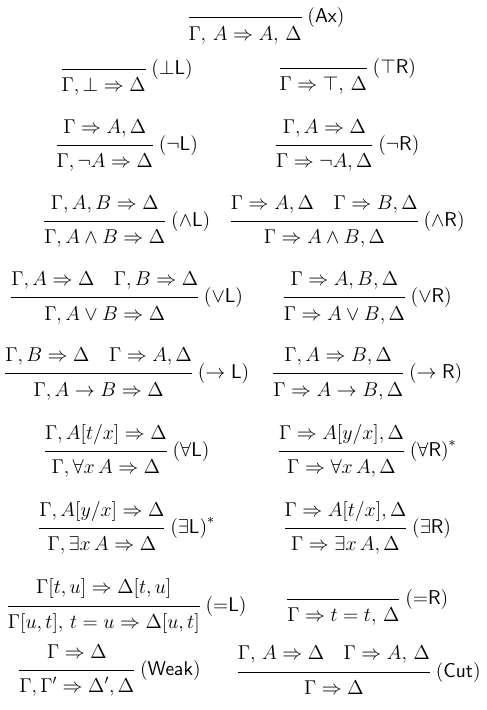
\includegraphics[width=\textwidth]{sequent2.png}
\end{minipage}
\begin{minipage}[t][][t]{0.5\textwidth}
\textbf{Computable partial functions:}\\
The set of computable partial functions $X$ is the smallest set, such that\\
1. $X$ contains $Z$, $s$ and $u_i^k$, defined by $Z(n) = 0$, $s(n) = n+1$,
$u_i^k(n_1, \ldots, n_k) = n_i$\\
2. If $f$ of arity $k$ and $g_1$, \ldots, $g_k$ or arity $\ell$ are in $X$, then so is the
$f \circ (g_1, \ldots, g_k)$, defined by
$f \circ (g_1, \ldots, g_k)(n_1, \ldots, n_\ell) = f(g_1(n_1, \ldots, n_\ell), \ldots, g_k(n_1, \ldots, n_\ell))$. \\
3. If $f$ of arity $k$ and $g$ of arity $k+2$ are in $X$, then so is $R_{fg}$ of arity $k+1$, defined recursively by
$R_{fg}(n_1, \ldots, n_k, 0) = f(n_1, \ldots, n_k)$ and
$R_{fg}(n_1, \ldots, n_k, n+1) = g(n_1, \ldots, n_k, n, R_{fg}(n_1, \ldots, n_k))$. \\
4. If $f$ of arity $k+1$ is in $X$ then so is $\mu f$ of arity $k$, defined by
$\mu f(n_1, \ldots, n_k) = $ the least such $n$ that $f(n_1, \ldots, n_k, n) = 0$ and
all $f(n_1, \ldots, n_k, i)$ are defined for $i < n$, if such $n$ exists. Otherwise undefined.  \\
Bullets 1 -- 3 are the definition of a computable function (not partial).
From exercises we know that: $+, \text{konst}, \dot{-}, \max, \min, == 0, != 0, \leq, ==, \sum_{n \leq n_0}, \prod_{n \leq n_0}$, partitional cases, are all computable.
\end{minipage}
% Sam uno je neki z relacijo? Ampak a ni mal nad tem, tud def. za funkcijo? haha
% mislm, je isto, ampak mors tukaj namesto $f$ pisat realcijo, kii predstavlja $f$
% nisem pisal :)
\hspace*{\fill} Avtorji: Vesna Iršič, Jure Slak, Anja Petković, Žiga Lukšič

\end{document}
% vim: syntax=tex
% vim: spell spelllang=sl
% vim: foldlevel=99
% Latex template: Jure Slak, jure.slak@gmail.com
